\documentclass[9pt]{beamer}
\mode<presentation>
{
  \usetheme{Boadilla}       % or try default, Darmstadt, Warsaw, ...
  \usecolortheme{beaver} % or try albatross, beaver, crane, ...
  \usefonttheme{serif}    % or try default, structurebold, ...
  \setbeamertemplate{navigation symbols}{}
  \setbeamertemplate{caption}[numbered]
} 
\setbeamertemplate{footline}
{
  \leavevmode%
  \hbox{%
  \begin{beamercolorbox}[wd=.35\paperwidth,ht=2.25ex,dp=1ex,center]{author in head/foot}%
    \usebeamerfont{author in head/foot}{Andrés Cadena (UNAL)}
  \end{beamercolorbox}%
  \begin{beamercolorbox}[wd=.37\paperwidth,ht=2.25ex,dp=1ex,center]{title in head/foot}%
    \usebeamerfont{title in head/foot}{Sobolev Spaces}
  \end{beamercolorbox}%
  \begin{beamercolorbox}[wd=.28\paperwidth,ht=2.25ex,dp=1ex,center]{date in head/foot}{Febrary 14, 2025}
  \insertframenumber{} / \inserttotalframenumber\hspace*{2ex} 
  \end{beamercolorbox}}%
  \vskip0pt%
}
\def\Xint#1{\mathchoice
{\XXint\displaystyle\textstyle{#1}}%
{\XXint\textstyle\scriptstyle{#1}}%
{\XXint\scriptstyle\scriptscriptstyle{#1}}%
{\XXint\scriptscriptstyle\scriptscriptstyle{#1}}%
\!\int}
\def\XXint#1#2#3{{\setbox0=\hbox{$#1{#2#3}{\int}$ }
\vcenter{\hbox{$#2#3$ }}\kern-.6\wd0}}
\def\ddashint{\Xint=}
\def\dashint{\Xint-}

\newcommand{\norma}[1]{{\left\vert\kern-0.25ex\left\vert\kern-0.25ex\left\vert #1 
    \right\vert\kern-0.25ex\right\vert\kern-0.25ex\right\vert}}


%%%%%%%%%%%%%%%%%%%%%%%%%%%%%%%%%%%%%%%%%%%%%%%%%%%%%%%%%%%%%%%%%%%%%%%%%%%%%%%%%%%%%%%%%%%%%%%%%%%%%%%%%%


%%%%%%%%%%%%%%%%%%%%%%%%%%%%%%%%%%%%%%%%%%%%%%%%%%%%%%%%%%%%%%%%%%%%%%%%%%%%%%%%%%%%%%%%%%%%%%%%%%%%%%%%%%

\DeclareMathOperator{\dist}{dist}
\DeclareMathOperator{\supp}{supp}

%%%%%%%%Tikz stuff
\usepackage{tikz} 
\usepackage{pgfplots}
\usepackage{hyperref}
\usepackage{ upgreek }
\usepackage{enumitem}
\usepackage{enumerate}
\usepackage{tcolorbox}
\usetikzlibrary{intersections, pgfplots.fillbetween}
\usepackage{tikz-3dplot}
\pgfplotsset{compat=1.7}
\usetikzlibrary{patterns}
%%%%%%%%%%%%%%%%%%%%%%%%%%%%%%%%%%%%%%%%%%%%%%

\usepackage{natbib}
\setcitestyle{year,open={(},close={)}}

%Simbolo demostración
\newcommand{\heart}{\begin{tikzpicture}[scale=0.001cm,rotate=180]
\fill[black] (0,0) 
        .. controls (0,-0.5) and (0.3,-1.8) .. (2,-2)
        .. controls (4.2,-2) and (5.5,0) .. (5.5,3)
        .. controls (5.5,5.5) and (3.5,7.5) .. (0,10)
        .. controls (-3.5,7.5) and (-5.5,5.5) .. (-5.5,3)
        .. controls (-5.5,0) and (-4.2,-2) .. (-2,-2)
        .. controls (-0.3,-1.8) and (0,-0.5) .. (0,0);
\end{tikzpicture}}

\newcommand{\demostrado}[0]{ \begin{flushright} $\heart{}$ \end{flushright}}

%sagetex
%\usepackage{sagetex}

\AtBeginSection[]
  {
     \begin{frame}<beamer>
     \frametitle{Content}
     \tableofcontents[currentsection]
     \end{frame}
  }
  
 
  
  
%%%%%%%%%%%%%%%%%%%%%%%%%%%%%%%%%%%%%%%%%%%%%%%%%%%%%%%%%%%%%%%%%%%%%%%%%%%%%%%%%%%%%%%%%%%%%%%%%%%%%%%%%%%%%%%%%%%%%%%%%%%%%%%%%%%%%%%New commands

\newcommand{\sech}{\operatorname{sech}}
%\DeclareMathOperator{\supp}{supp}
\usepackage{xcolor}
\usepackage{enumitem}
\definecolor{mirojo}{RGB}{160,0,0}
\setbeamercolor{section number projected}{bg=mirojo,fg=white}
\setbeamercolor{subsection number projected}{bg=mirojo,fg=white}
\setlist[enumerate]{label=\textcolor{mirojo}{\arabic*.}}
\setbeamercolor{block title}{bg=mirojo,fg=white}
\setbeamercolor{block body}{bg=mirojo!20,fg=black}
\providecommand{\norm}[1]{\left\|#1\right\|}


%%%%%%%%%%%%%%%%%%%%%%%%%%%%%%%%%%%%%%%%%%%%%%%%%%%%%%%%%%%%%%%%%%%%%%%%%%%%%%%%%%%%%%%%%%%%%%%%%%%%%%%%%%%%%%%%%%%%%%%%%%%%%%%%%%%%%%%%%%%%%%%%%%%%%%%%%%%%%%%%%%%%%%%%%%%


\title{Estimación tipo conmutador para transformadas de Hilbert y derivadas fraccionarias.}
\author{\texorpdfstring{ 
Andrés David Cadena Simons \\
Universidad Nacional de Colombia, Bogotá}{A}}

\institute{ }
\date{\footnotesize Julio 29, 2025}

\setbeamertemplate{itemize items}[default]
\setbeamertemplate{enumerate items}[default]

\begin{document}

\begin{frame}
  \titlepage

\end{frame}


\begin{frame}{Content}
  \tableofcontents
\end{frame}

\section{Resúmen.}

\begin{frame}{Resúmen}
  En este trabajo se estudia una estimación de conmutador para el operador $H_x D_x^\alpha$, compuesto por la transformada de Hilbert y una derivada fraccionaria. Específicamente, se demuestra que
  \begin{align*}
    \| [H_x D_x^\alpha, g] D_x^\beta f \|_{L^p} \lesssim \| \partial_x g \|_{L^\infty} \cdot \|f\|_{L^p},
  \end{align*}
  donde $\alpha + \beta = 1$ y $1 < p < \infty$.
  \cite{zbMATH07319426}.
\end{frame}

\section{Introducción.}

\begin{frame}{Estimación}
  \begin{block}{Estimación tipo conmutador no local}
    Sea $1 < p < \infty$, $0 < \alpha, \beta \leq 1$, tal que $\alpha + \beta = 1$. Entonces
    \begin{align*}
      \norm{D_x^{\alpha} [H_x, g] D_x^{\beta} f}_{L^p(\mathbb{R})} \lesssim_{p,\alpha,\beta} \norm{\partial_x g}_{L^\infty(\mathbb{R})}\norm{f}_{L^p(\mathbb{R})}, 
    \end{align*}
    para toda función $g$ suave con derivada acotada y toda $f \in \mathcal{S}(\mathbb{R})$.
  \end{block}
\end{frame}

\section{Preliminares.}

\begin{frame}{}
  Recordamos que la transformada de Hilbert $H_x$ está definida en la transformada de Fourier como
  \begin{align*}
    \hat{H_x f}(\xi) = -isgn(\xi) \hat{f}(\xi). 
  \end{align*}  
\end{frame}

\begin{frame}{}
  Además, las derivadas fraccionarias están dadas por el operador
  \begin{align*}
    \hat{D_x^s f}(\xi) = |\xi|^s \hat{f}(\xi), \qquad s \in \mathbb{R}. 
  \end{align*}
\end{frame}

\begin{frame}{}
  También usaremos las proyecciones de Littlewood–Paley $P^x_N$ definidas por
  \begin{align*}
    \hat{P^x_N f}(\xi) = \psi_N(\xi) \hat{f}(\xi), 
  \end{align*}
  donde $\psi_N(\xi)$ es un multiplicador suave con soporte en frecuencias de orden $|\xi| \sim N$, con $N$ número diádico.
\end{frame}

\begin{frame}{}
  \begin{block}{Fefferman–Stein}
    Sea $f = (f_j)_{j=1}^{\infty}$ una secuencia de funciones localmente integrables en $\mathbb{R}$. Si $1 < p < \infty$, entonces
    \begin{align*}
      \norm{(Mf_j)_{l^2}}_{L^p} \leq C_p \norm{(f_j)_{l^2}}_{L^p}, 
    \end{align*}
    donde $M$ denota la función maximal de Hardy–Littlewood.
  \end{block}
\end{frame}

\begin{frame}
  \begin{block}{Estimación tipo Calderón}
    Para $l + m \geq 1$, se tiene
    \begin{align*}
      \norm{\partial_x^l [H_x, g] \partial_x^m f}_{L^p} \lesssim \norm{\partial_x^{l + m} g}_{L^\infty} \norm{f}_{L^p}. 
    \end{align*}
  \end{block}
\end{frame}

\section{Demostración}

\begin{frame}{Demostración}
  \subsection*{Expresión integral del conmutador en Fourier}
  Note que por la definición de conmutador se tiene que
  \begin{align*}
    [H_x, g] D_x^\beta f = H_x(g D_x^\beta f) - g H_x D_x^\beta f. 
  \end{align*}
  Aplicamos la derivada fraccionaria
  \begin{align*}
    D_x^\alpha [H_x, g] D_x^\beta f = D_x^\alpha H_x(g D_x^\beta f) - D_x^\alpha (g H_x D_x^\beta f). 
  \end{align*}
\end{frame}

\begin{frame}{}
  Usando su expresión como multiplicador se tiene que
  \begin{align*}
    \hat{\left(D_{x}^{\alpha}H_{x}(gD_{x}^{\beta}f)\right)}(\xi)&=(2\pi i)^{|\alpha|}|\xi|^{\alpha}(-i sgn(\xi))\hat{gD_{x}^{\beta}f}(\xi),\\
    &=(2\pi i)^{|\alpha|+|\beta|}(-i)\int_{-\infty}^{\infty}sgn(\xi)|\xi|^{\alpha}|\xi-\eta|^{\beta}\hat{g}(\eta)\hat{f}(\xi-\eta)\, d\eta.
  \end{align*}
\end{frame}

\begin{frame}
  De manera similar se puede llegar a que
  \begin{align*}
    \hat{\left( D_{x}^{\alpha}gH_{x}D_{x}^{\beta}f \right)}(\xi)&=(2\pi i)^{|\alpha|+|\beta|}(-i)\int_{-\infty}^{\infty}sgn(\xi-\eta)|\xi|^{\alpha}|\xi-\eta|^{\beta}\hat{g}(\eta)\hat{f}(\xi-\eta)\, d\eta.
  \end{align*}
\end{frame}

\begin{frame}
  Siendo así, juntando ambas expresiones y realizando los cambios de variables $\eta=\xi_{1}$ y $\xi_{2}=\xi-\eta$, es decir $\xi_{1}+\xi_{2}=\xi$ podemos verificar que
  \begin{align*}
    \hat{\left( D_{x}^{\alpha}\left[ H_{x},g \right]D_{x}^{\beta}f \right)}(\xi_{1}+\xi_{2})&=(2\pi i)^{|\alpha|+|\beta|}(-i)\int_{-\infty}^{\infty}(sgn(\xi_{1}+\xi_{2})-sgn(\xi_{2}))|\xi_{1}+\xi_{2}|^{\alpha}|\xi_{2}|^{\beta}\hat{g}(\xi_{1})\hat{f}(\xi_{2})\, d\xi_{1}.
  \end{align*}
  Lo que nos permite afirmar que
  \begin{align*}
    (2\pi i)^{|\alpha|+|\beta|}(-i)\int_{-\infty}^{\infty}\int_{-\infty}^{\infty}(sgn(\xi_{1}+\xi_{2})-sgn(\xi_{2}))|\xi_{1}+\xi_{2}|^{\alpha}|\xi_{2}|^{\beta}\hat{g}(\xi_{1})\hat{f}(\xi_{2})e^{2\pi ix(\xi_{1}+\xi_{2})}\, d\xi_{1}d\xi_{2}. 
  \end{align*}
\end{frame}

\begin{frame}{}
  Note que el integrando solamente es igual a $0$ cuando $sgn(\xi_{1}+\xi_{2})-sgn(\xi_{2})=0$, es decir cuando $(\xi_{1}+\xi_{2})(\xi_{2})>0$, por lo que solo estaremos interesados en estudiar cuando $(\xi_{1}+\xi_{2})(\xi_{2})<0$, es decir
  \begin{align*}
    \begin{cases}
      \xi_{2}>0, &\text{ entonces } \xi_{1}<-\xi_{2} \text{,} \\
      \xi_{2}<0, &\text{ entonces } \xi_{1}>-\xi_{2}.
    \end{cases}
  \end{align*}
  \begin{center}
    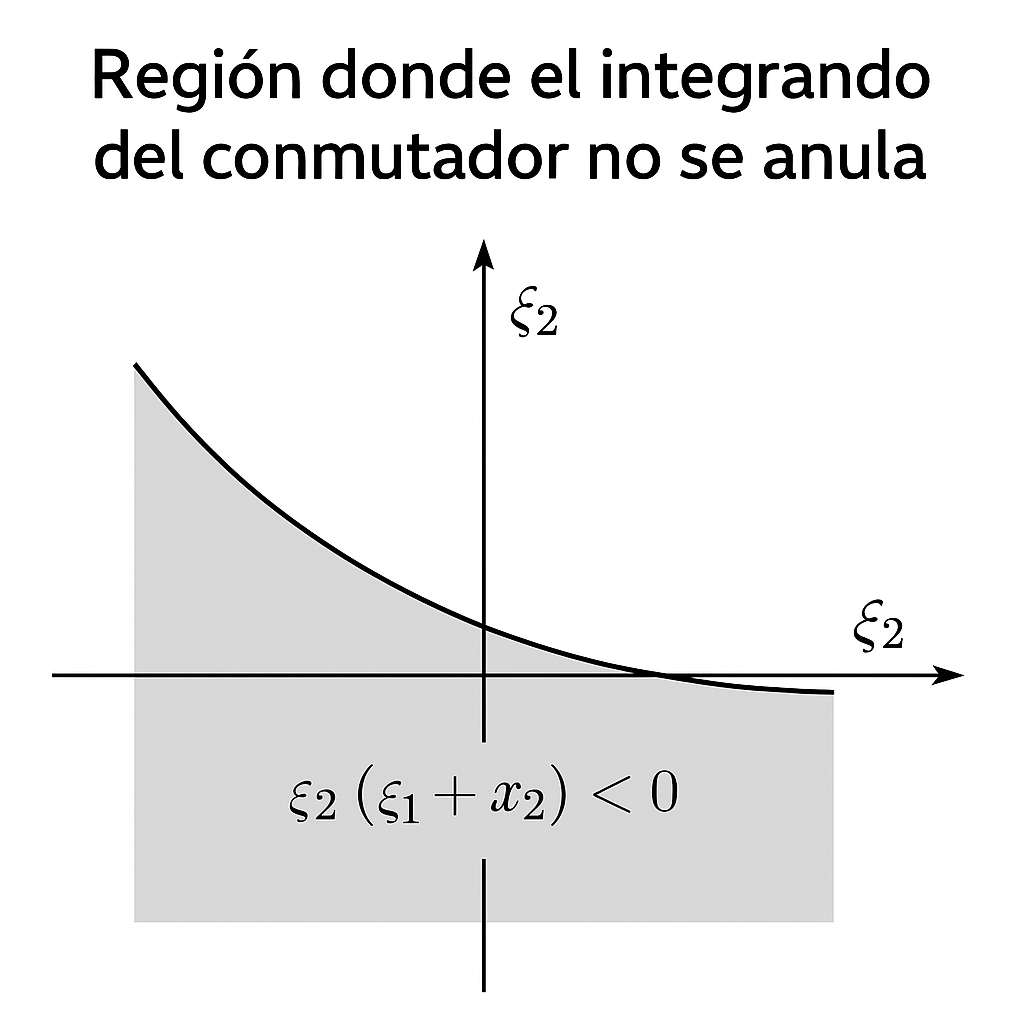
\includegraphics[scale=0.15]{Diagrama de conmutador en 2D.png}
  \end{center}
\end{frame}

\begin{frame}{}
  \begin{align*}
    D_x^\alpha [H_x, g] D_x^\beta f &=H_{x}\left( \sum_{N>0}D^{\alpha}(P_{N}^{x}gP_{\ll N}^{x}D_{x}^{\beta}f) \right)-\sum_{N>0}D^{\alpha}(P_{N}^{x}gP_{\ll N}^{x}H_{x}D_{x}^{\beta}f)\\
    &\phantom{=}+H_{x}\left(\sum_{N>0}D^{\alpha}(P_{N}^{x}g\tilde{P}_{N}^{x}D_{x}^{\beta}f) \right)-\sum_{N>0}D^{\alpha}(P_{N}^{x}g\tilde{P}_{N}^{x}H_{x}D_{x}^{\beta}f),\\
    &= A_1 + A_2 + A_3 + A_4, 
  \end{align*}
\end{frame}

\section{Bibliografía.}

\begin{frame}[allowframebreaks]
	\frametitle{Bibliography.}
	
	
	\bibliographystyle{authordate1} 
  \nocite{*}
	%  \bibliographystyle{plain}
	\bibliography{references}
\end{frame}


%%%%%%%%%%%%%%%%%%%%%%%%%%%%%%%%%%%%%%%%%%%%%%%%%%%%%%%%%%%%%%%%%%%%%%%%%%%%%%%%%%%%%%%%%%%%%%%%%%%%%%%%%%%%%%%%%%%%%%%%%%%%%%%%%%%%%%

\begin{frame}
\begin{center}
  \Huge {\color{red} Gracias por su atención.} 
  \begin{center}
	  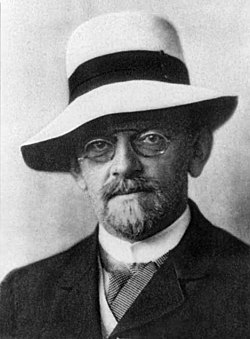
\includegraphics[scale=0.5]{Hilbert.jpg}
  \end{center}
\end{center}
    
\end{frame}
\begin{frame}{Board}
\end{frame}

\end{document}
